%%%%%%%%%%%%%%%%%%%%%%%%%%%%%%%%%%%%%%%%%%%%%%%%%%%%%%
\chapter{Integrated experimental strategy}
\label{integrated_experimental_strategy}
\graphicspath{{chapter_03/figures}{chapter_03/tables}}
%%%%%%%%%%%%%%%%%%%%%%%%%%%%%%%%%%%%%%%%%%%%%%%%%%%%%%


This chapter outlines the integrated experimental strategy adopted in this thesis, wherein each research question and objective - presented in Chapter \ref{general_introduction} - builds upon its predecessor to establish a proof of concept for medium-range predictions of areas at risk of flash floods across a continuous global domain (upper panel in Figure \ref{fig:integrated_experimental_strategy}). The integrated experimental strategy is here exemplified through the \textit{methodological decisions} underlying each research question and objective (lower panel in Figure \ref{fig:integrated_experimental_strategy}). Such decisions encompass three primary areas: the selection of appropriate data sources (Section \ref{integrated_experimental_strategy_data_requirements}), the formulation of the forecast verification strategy (Section \ref{integrated_experimental_strategy_verification_strategy}), and the strategy for developing a data-driven model to identify areas at risk of flash floods under imbalanced observational datasets (Section \ref{integrated_experimental_strategy_model_development_imbalanced_data}). 

\begin{figure}[htbp]
\centering
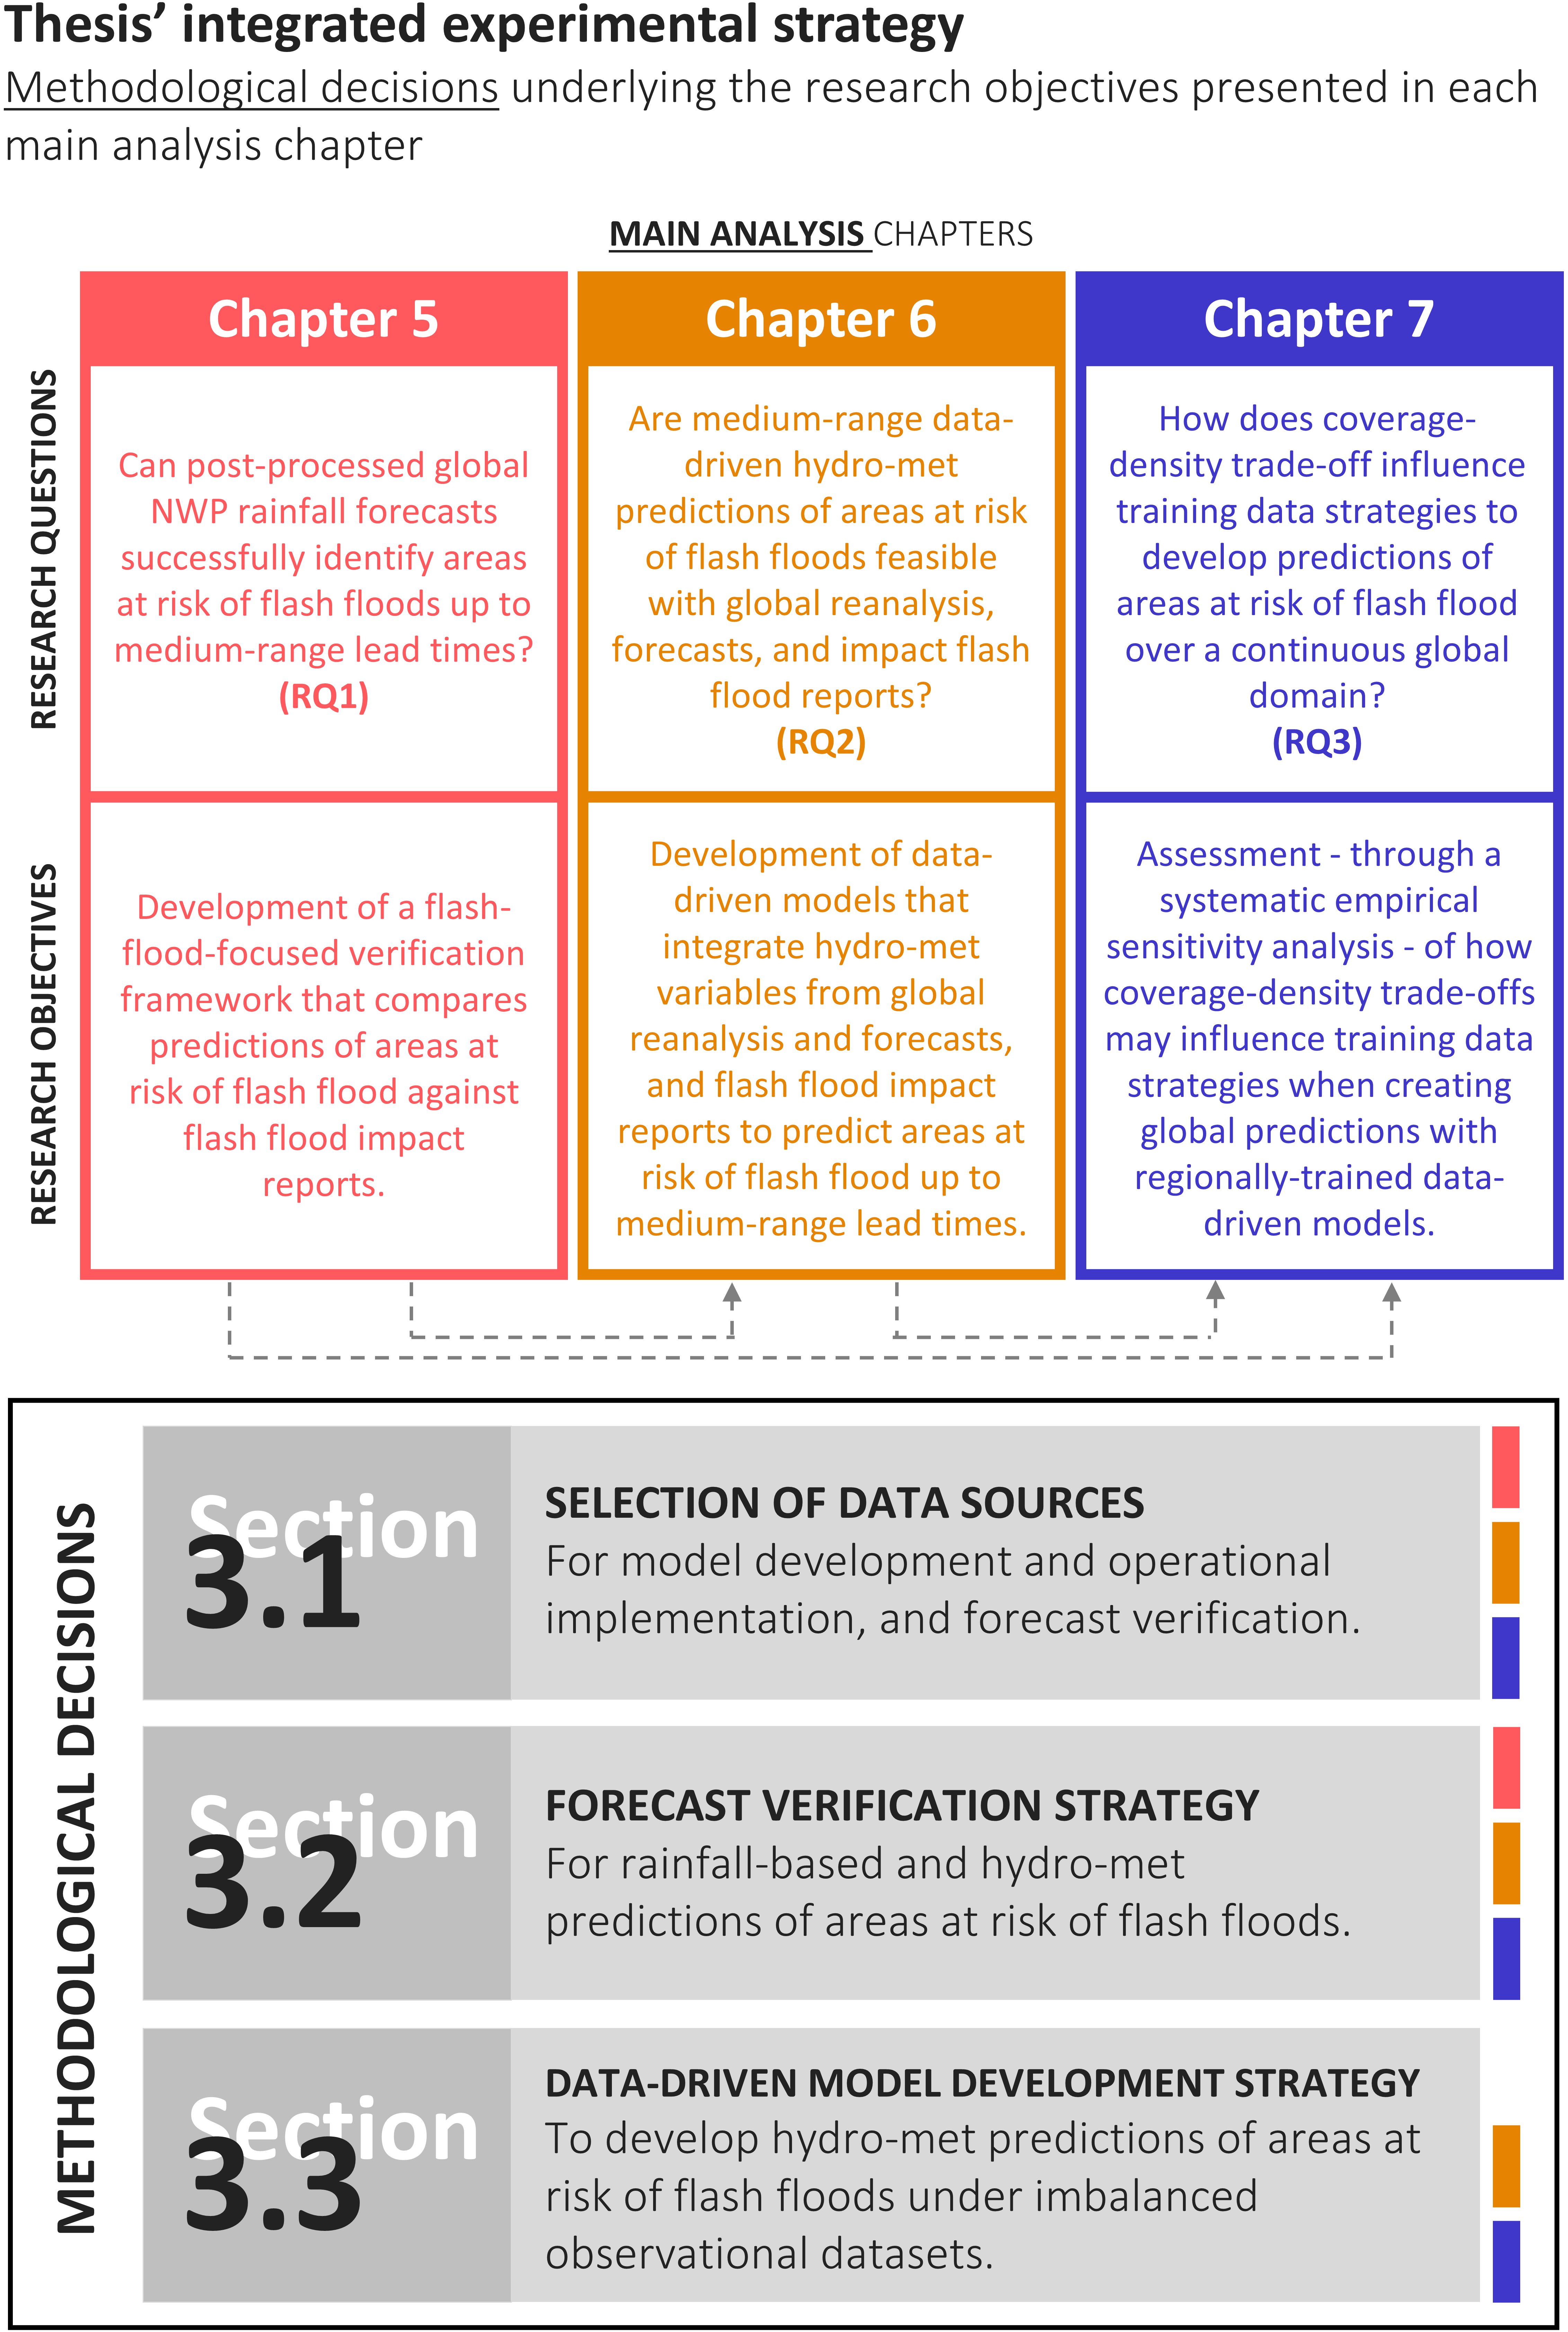
\includegraphics[width=\textwidth]{chapter_03/figures/integrated_experimental_strategy.png}
\caption{\textbf{Thesis' integrated experimental strategy.} The upper panel of the infographic reminds the reader about the hierarchical relationship between research questions RQ1 (addressed in the Main Analysis Chapter \ref{flash_flood_focused_verification_rainfall_based_ff}, card in pink), RQ2 (Main Analysis Chapter \ref{data_driven_flash_floods_short_medium_range}, card in yellow), and RQ3 (Main Analysis Chapter \ref{regional_to_global_training}, card in blue) and corresponding research objectives. The horizontal dashed arrows beneath each card indicate the cross-chapter information flow as introduced in Chapter \ref{general_introduction}. The lower panel of the infographic (within the solid black box) identifies the three core methodological decisions that inform the integrated experimental strategy: data source selection (Section \ref{integrated_experimental_strategy_data_requirements}), forecast verification strategy (Section \ref{integrated_experimental_strategy_verification_strategy}), and data-driven model development strategy (Section \ref{integrated_experimental_strategy_model_development_imbalanced_data}). The coloured indicators on the right of each grey card identify the main analysis chapter in which each methodological decision was applied.}
\label{fig:integrated_experimental_strategy}
\end{figure}


%%%%%%%%%%%%%%%%%%%%%%%%%%%%%%%%%%%%%%%%%%%%%%%%%%%%%%%%%%
\section{Data requirements and selection}
\label{integrated_experimental_strategy_data_requirements}

The development of a flash flood prediction system necessitates careful consideration of data requirements across all methodological components, e.g. model development, forecast verification (at different lead times), and future operational implementation. This section outlines the criteria for selecting the required data to develop a proof of concept of a system that produces medium-range forecasts of areas at risk of flash floods over a continuous global domain (Section \ref{integrated_experimental_strategy_data_requirements_selection_criteria}) and provides the final selection within available sources (Section \ref{integrated_experimental_strategy_data_requirements_final_selection}). 


\subsection{Requirements for data selection}
\label{integrated_experimental_strategy_data_requirements_selection_criteria}

\subsubsection{Requirements for observational data}

Given \marginpara{Requirement for observational data n.1: spatio-temporal accuracy of reported flash flood events} that flash floods are rapid-onset, localised events typically occurring in small catchments, observational datasets must accurately capture both the location and timing of each event, alongside quantifying the spatio-temporal uncertainty associated with each record. This precision is essential for developing a robust flash-flood-focused verification framework (RQ1), where grid-based assessments require accurate spatial assignment of events to model grid cells. Furthermore, precise spatio-temporal information enables prediction systems — whether data-driven or physics-based — to establish meaningful relationships between local meteorological conditions and flash flood occurrence, thereby capturing the fine-scale processes that govern these rapid-onset events (RQ2 and RQ3).

The \marginpara{Requirement for observational data n.2: long, complete, and consistent timeseries of reported events.} rarity of flash flood events necessitates extensive temporal coverage to accumulate an adequate number of flash flood events for robust forecast verification (RQ1 to RQ3) and data-driven model training (RQ2). Additionally, consistent reporting standards across the considered spatial domain ensure unbiased verification and prevent the introduction of artificial patterns during model training. Moreover, consistent reporting standards would facilitate sensitivity analyses for expanding regional training to global scales, should suitable global databases not be available (RQ2).

\subsubsection{Requirements for hydro-meteorological forecasts}

To \marginpara{Requirement for hydro-meteorological forecasts  n.1: consistent forecasts spatial resolution through the lead time horizon} analyse forecast predictability from short-range (i.e., up to day 1; RQ1 and RQ2) to medium-range lead times (up to day 5; RQ1 and RQ3), a system providing consistent spatial resolution across all lead times would be preferable. Varying resolutions would compound extrinsic uncertainties with those intrinsic ones present in flash flood predictions, arising from both the chaotic nature of flash-flood-generating rainfall events and the complexity of the hydrological processes involved in flash flood generation. Hence, by employing consistent spatial resolution throughout, any lead-time-driven model performance degradation may reflect genuine predictability limits rather than dataset inconsistencies.

Due \marginpara{Requirement for hydro-meteorological forecasts  n.2: capability to represent flash-flood-triggering rainfall events} to their coarse resolution and parametrisation schemes of convective systems, raw global NWP model outputs systematically underestimate localised rainfall extremes, which are critical for flash flood generation. Consequently, both the verification of areas at risk of flash floods (RQ1 to RQ3) and the training of machine learning models for predicting such areas at risk of flash floods (RQ2) require rainfall estimates that can identify flash-flood-triggering rainfall events. 

Whilst \marginpara{Requirement for hydro-meteorological forecasts  n.3: Global coverage} the proof of concept proposed in this thesis focuses in the creation (RQ2 and RQ3) and verification (RQ1 to RQ3) of predictions of areas at risk of flash floods over the CONUS, the methodology must support global extension. This requirement necessitates globally consistent datasets without regional discontinuities, typically provided by global NWP model outputs.


\subsection{Proposed data sources}
\label{integrated_experimental_strategy_data_requirements_final_selection}

\subsubsection{Observational dataset}

The \marginpara{Choice of observational data: impact-based reports vs gauge-based measurements} observational data available for this thesis fall into two main categories: impact-based reports and gauge-based measurements. The choice of using impact-based reports rather than gauge-based measurements reflects this thesis's objective to predict areas at risk of both fluvial flash floods - occurring within river channels - and pluvial flash floods - resulting from inadequate urban drainage systems or surface runoff accumulation, including areas away from river channels. Discharge gauges capture only fluvial flash floods, whilst impact databases enable the identification of both fluvial and pluvial events. Furthermore, gauge-based observations systematically underestimate flash flood frequency due to a sparse observational network and the tendency for flashy catchments to remain ungauged \citep{Gaume_2009, Gaume_2016}. Although impact databases are subject to reporting biases — notably those related to population density \citep{Marjerison_2016} — they provide the most feasible approach for developing and verifying continental-scale predictions of areas at risk of flash floods.

This \marginpara{Chosen impact database - NOAA's Storm Event Database over CONUS - and its comparison to alternative databases} thesis employs NOAA's Storm Events Database\footnote{For more details, refer to Section \ref{storm_event_database} in Chapter \ref{datasets}} over the CONUS as the primary observational data source. Compared to other impact databases, the Storm Event Database represents the most comprehensive and systematically maintained record of flash flood impacts available at a continental scale, containing detailed spatio-temporal information from 1996 to the present, including location and reporting time uncertainties for each event. The database's consistent reporting standards across all US states, maintained through NOAA quality control procedures, reduce, though do not eliminate, reporting inconsistencies. Such spatial consistency enables robust model development and forecast verification across CONUS' diverse hydro-climatic regions, while also facilitating sensitivity analyses for expanding regional training to a global scale. Whilst alternative databases exist, they present significant limitations. ESSL's ESWD database lacks direct flash flood reports, recording only "extreme rainfall" events \citep{Dotzek_2009}. Such reports are usually considered as proxies for flash flooding. However, as stated in Chapter \ref{general_introduction}, a direct correlation between rainfall events and flash flood generation is not assumed in this thesis. Furthermore, ESWD presents a spatial bias with disproportionately high observation density over Germany, where ESSL is based \citep{Dotzek_2009}. Such a difference is inconsistent with the literature, which provides no evidence of higher flash flood frequency in Germany relative to neighbouring countries \citep{Gaume_2009}. Hence, if ESWD were the primary observational dataset, errors in the spatial representation of areas at risk of flash floods might be introduced during model training and forecast verification. Global impact databases such as EM-DAT and DesInventar contain an insufficient number of flash flood records due to their inclusion criteria and the inherent difficulty of systematically documenting small-scale events worldwide \citep{Panwar_2020}.

\subsubsection{Hydro-meteorological forecasts}

The \marginpara{Chosen reanalysis and forecasting system for hydrological and static parameters - ERA5} selection of ERA5-related datasets\footnote{For more details, refer to Section \ref{datasets_era5} in Chapter \ref{datasets}} (both reanalysis and medium-range forecasts) reflects a deliberate strategy to maintain consistency across the three research components of this thesis. ERA5 provides a long-term (from the 1940s to the present), high-quality reconstruction of hydrological and static fields over a continuous global domain \citep{Hersbach_2020}.  This temporal extent ensures sufficient historical data to capture the full spectrum of meteorological conditions associated with flash flood events, including rare, extreme scenarios that may occur infrequently within shorter time series. The global coverage and uniform spatial resolution of ERA5 eliminate boundary effects and regional inconsistencies that could compromise model transferability across different geographical domains. Furthermore, the availability of medium-range predictions with the same spatial resolution as the reanalysis data used during model training facilitates the analysis of forecast predictability with minimum disruption due to fine-tuning of low-resolution training datasets to higher-resolution forecasts, as seen in other data-driven systems \citep{Lang_2024}.

While \marginpara{Chosen reanalysis and forecasting system to represent localised extreme rainfall - ERA5-ecPoint} ERA5 provides a consistent dataset for training and prediction across space and time, its coarse resolution (31 km) renders raw ERA5 rainfall estimates unsuitable for flash flood applications. Localised rainfall peaks tend to be underestimated in the case of large-scale rainfall (whether from stratiform rainfall or large convective systems) or absent in the case of isolated convection. Hence, the rainfall estimates used in this thesis for training, model development, and verification come from the post-processed ERA5 rainfall estimates with the ecPoint methodology (ERA5-ecPoint\footnote{For more details, refer to Section \ref{datasets_era5_ecpoint} in Chapter \ref{datasets}}). ERA5-ecPoint provides a probabilistic distribution of the localised extreme rainfall estimates that might be observed by rain gauges within model grid-boxes, being, therefore, more representative of point-scale rainfall's local maxima.


%%%%%%%%%%%%%%%%%%%%%%%%%%%%%%%%%%%%%%%%%%%%%%%%%%%%%%%%%%%%%%
\section{Forecasts verification strategy}
\label{integrated_experimental_strategy_verification_strategy}

\subsection{Requirements for robust evaluation of probabilistic forecasts predicting rare events}

The \marginpara{Requirement n.1 for robust evaluation of probabilistic forecasts predicting rare events: objective verification of both features of probabilistic forecasts - reliability and discrimination ability} operational utility of probabilistic forecasts - in this case for the prediction of areas at risk of flash floods - relies on the concurrent high performance in both \textit{reliability} and \textit{discrimination ability}. Both features are defined for events exceeding a \textit{verifying threshold} (VT, in the same forecast units) with probabilities higher than a specific probability threshold (PT, in \%). Reliability measures whether, for a specific probability bin, the chosen VT is predicted with a probability that equals the average frequency at which such an event is observed within that probability bin. Discrimination measures the ability of the forecasts to distinguish between situations that lead to events exceeding the VT, at specific PTs, and those that do not. As shown in \citet{Pillosu_2025} for rainfall, forecasts exhibiting high discrimination ability may nonetheless yield uncalibrated probabilities. Conversely, forecasts that achieve good reliability but exhibit poor discrimination provide minimal operational utility as they cannot effectively identify when conditions deviate from climatological norms to signal heightened event likelihood. Hence, explicit examination of both features is needed through \textit{objective verification}, i.e., through the use of appropriate statistical verification scores.

\textit{Overall} \marginpara{Requirement n.2 for robust evaluation of probabilistic forecasts predicting rare events: use of overall and breakdown scores} and \textit{breakdown} scores must be considered to ensure a thorough evaluation of forecast reliability and discrimination ability. Overall scores integrate performance across all PTs, providing valuable summaries for model comparison and evaluation. However, these aggregated metrics may mask critical performance variations at specific PTs through compensating errors across the probability spectrum. Moreover, operational applications may prioritise performance assessments at particular probability thresholds rather than uniform skill assessments. Hence, breakdown scores complement overall metrics by providing a granular performance assessment across discrete probability thresholds, thereby enabling complete characterisation of forecast utility.

When \marginpara{Requirement n.3 for robust evaluation of probabilistic forecasts predicting rare events: selection of appropriate metrics for rare events} evaluating predictions of binary outcomes (e.g., occurrence of yes- and non-events) for rare events, the difference between the number of cases falling into the "yes-event" and "non-event" classes may be large. In this case, one would say there is a \textit{class imbalance}, with the negatives typically outnumbering the positives (which are the events of interest, e.g., flash flood occurrence). Class imbalance may render traditional accuracy metrics meaningless, with forecasts predicting exclusively non-events achieving 99.8\% accuracy while providing no operational value \citep{Wilks_2020}. Accordingly, verification metrics must quantify the forecasts' capacity to identify rare yes-events. 

In \marginpara{Requirement n.4 for robust evaluation of probabilistic forecasts predicting rare events: subjective verification of specific case-studies} addition to analysing forecast performance through objective verification, it is argued that predictions should also be examined through \textit{subjective verification}. Provided there are enough observations for specific case studies, this type of analysis may be more effective than objective verification in differentiating forecast performance and predictability in specific cases of interest. Objective verification might indeed yield statistically weak results if the observational sample size is small. 


\subsection{Proposed forecasts verification strategy}

To \marginpara{Chosen (overall and breakdown) scores to assess reliability and discrimination ability: frequency bias and reliability diagrams, ROC curves and areas under the ROC} assess reliability and discrimination ability, this thesis will employ scores commonly used in the assessment of probabilistic weather forecasts \citep{Wilks_2020, Jolliffe_2012}. The \textit{frequency bias} will be used as an overall measure of reliability as it provides an estimate of systematic over- and under-prediction by comparing the predicted probabilities for an event with its observed frequency. \textit{Reliability diagrams} will extend this analysis by plotting observed frequencies against forecast probabilities for discrete probability bins, thereby revealing calibration issues at specific probability ranges. To assess discrimination ability, the Receiver Operating Characteristic (ROC) curve will be considered to assess the trade-off between hit rates and false alarm rates across different probability thresholds. The Area under the ROC curve (AUC-ROC) will then be considered as an overall measure of discrimination ability. Figure \ref{fig:forecast_evaluatio_strategy} - Objective Verification - lists the chosen verification scores, alongside the data processing (DP) pipeline required to transform raw observations and forecasts into the appropriate format to run the objective verification analysis.

\begin{figure}[htbp]
\centering
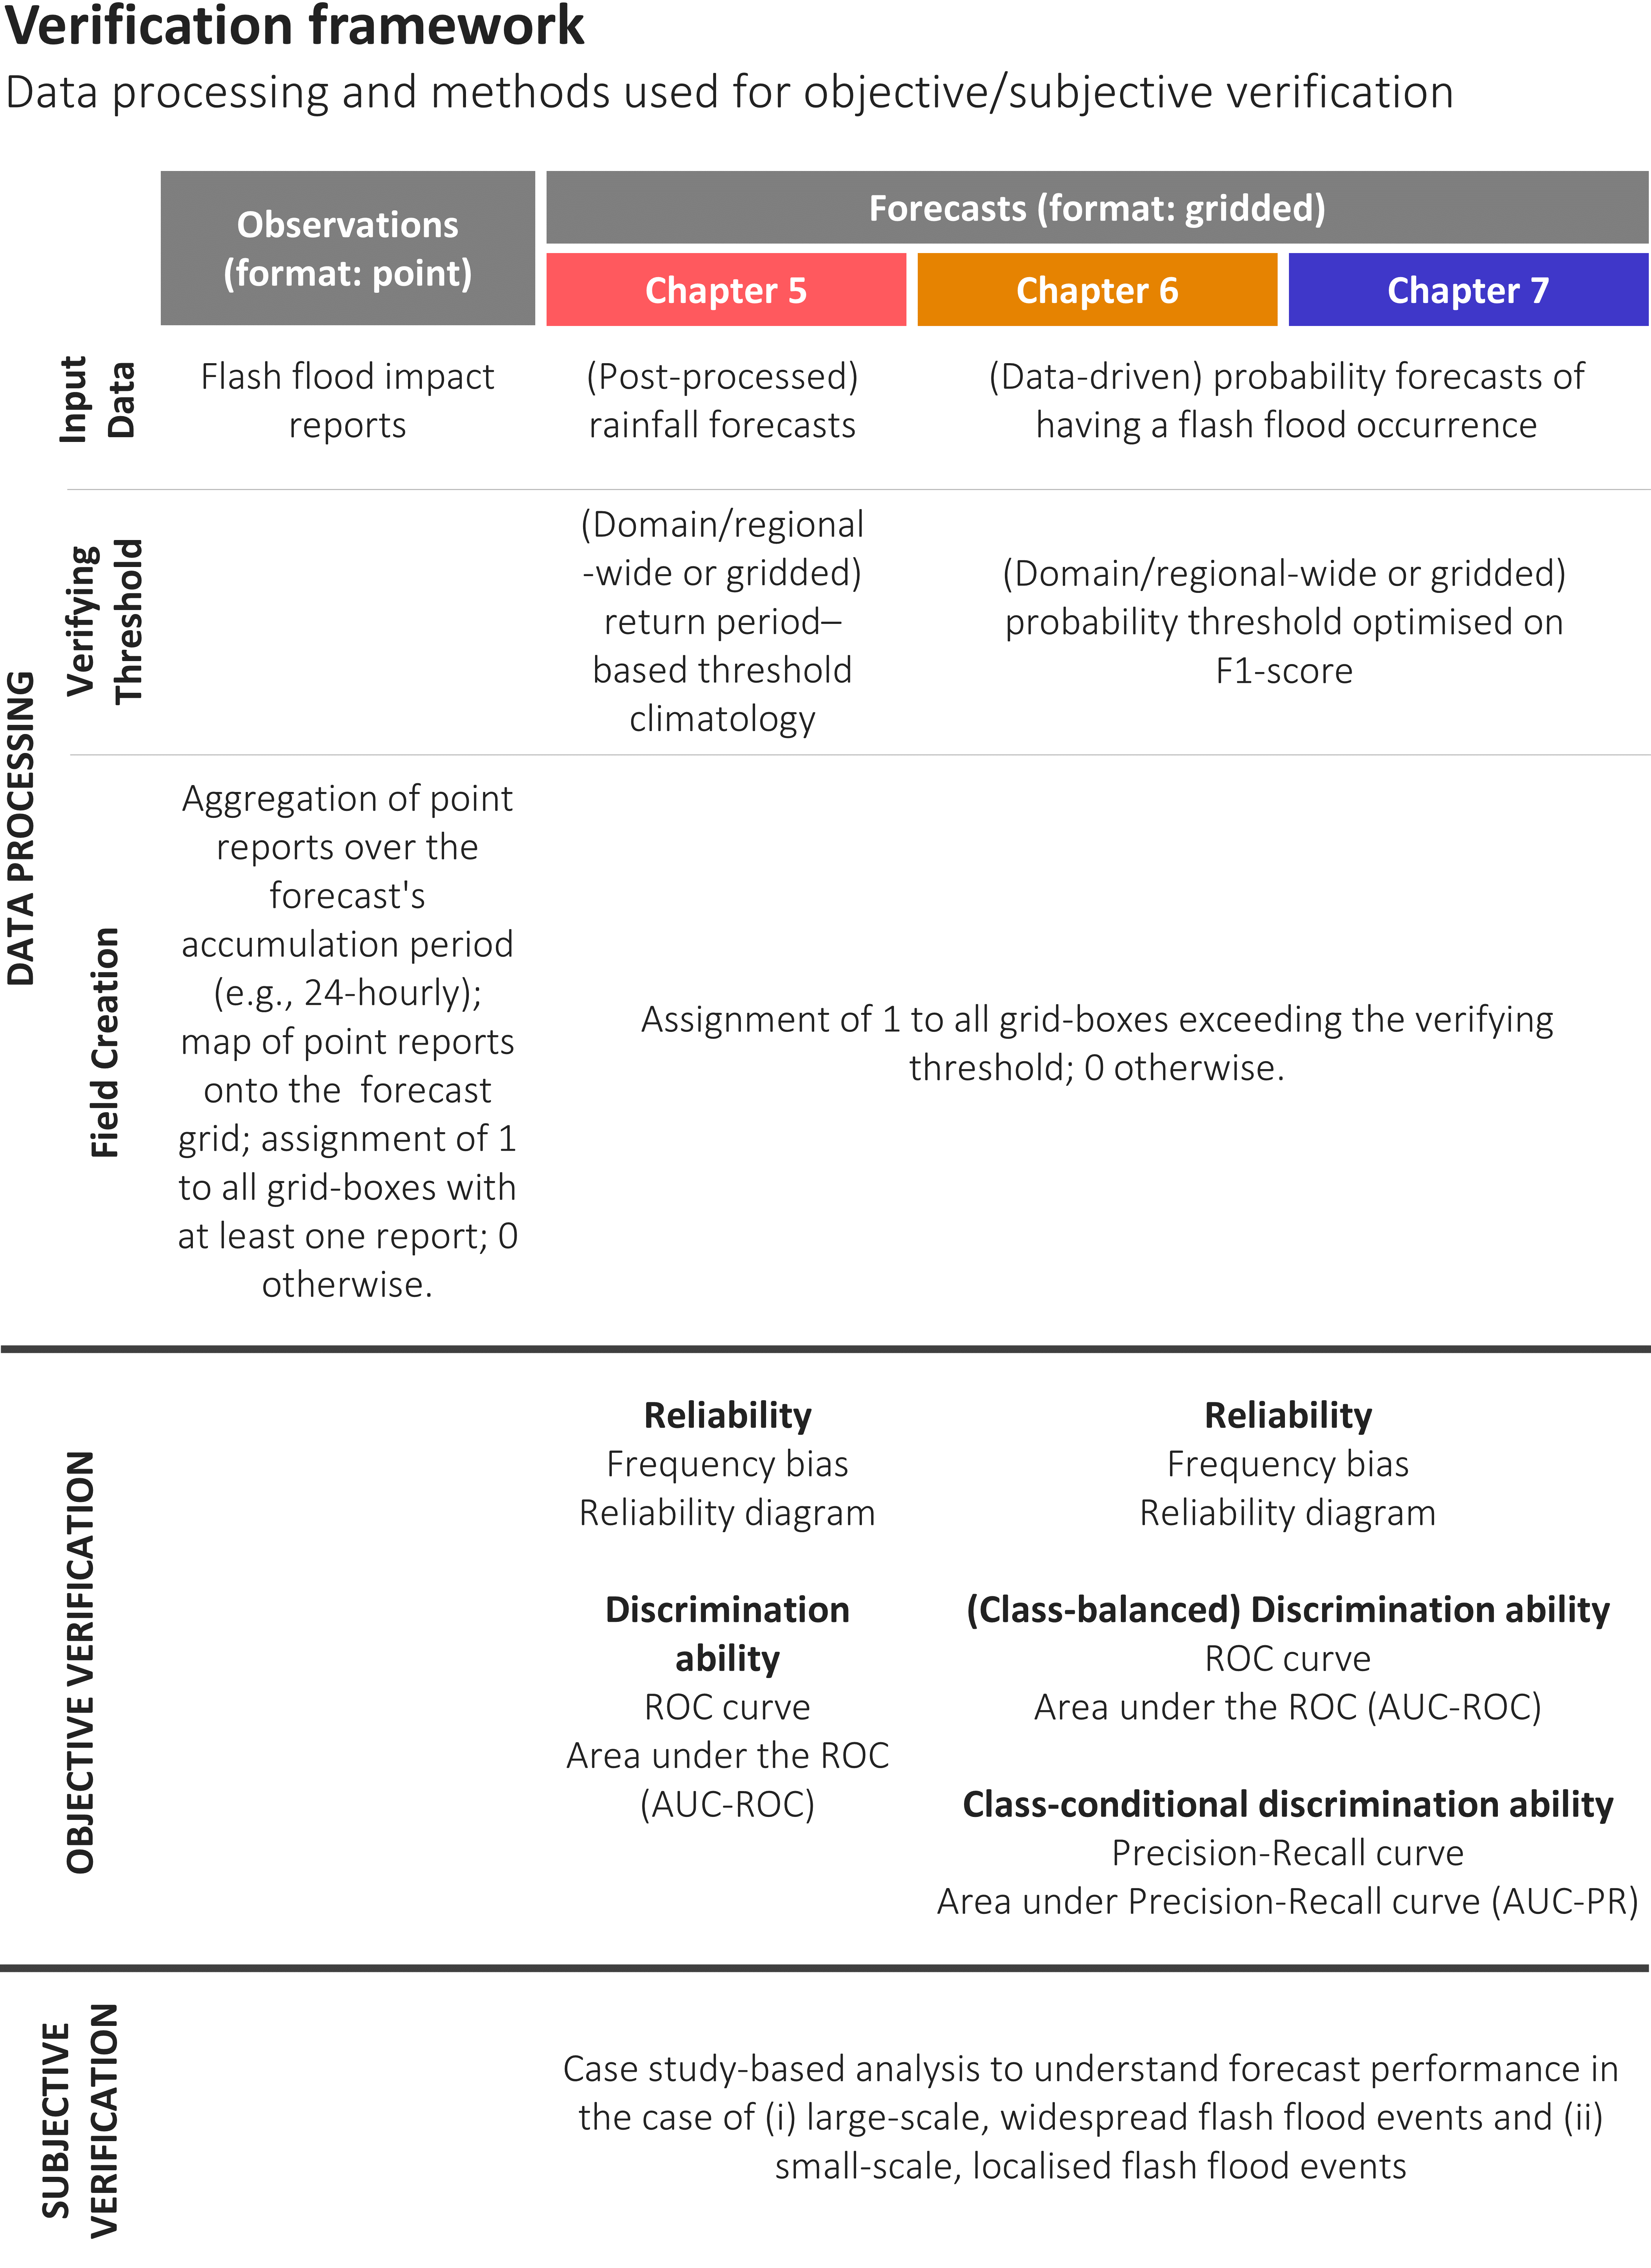
\includegraphics[width=\textwidth]{forecast_evaluation_strategy.png}
\caption{\textbf{Verification framework for objective and subjective evaluation of predictions of areas at risk of flash flood.} The infographic illustrates the initial data processing, showing how to prepare observations and forecasts, whether rainfall-based (as in Chapter 5) or probability-based (as in Chapter 6 and 7). The infographic also illustrates the scores used in the objective verification to assess forecast reliability (i.e., Frequency Bias and Reliability Diagrams) and discrimination ability (i.e., ROC curve and Area under the ROC), as well as discrimination ability for forecasts created under class imbalance (as in Chapter 6 and 7, i.e., Precision-Recall curve and Area under the Precision-Recall curve). Subjective verification employs case study analyses for both large-scale, widespread and small-scale, localised flash flood events.}
\label{fig:forecast_evaluatio_strategy}
\end{figure}

As \marginpara{Chosen robust metrics to assess forecasts for rare events} mentioned in the previous paragraph, ROC curves and AUC-ROC are commonly used to assess discrimination ability in hydro-meteorology. ROC curves are built from a contingency table (Figure \ref{fig:curve_roc_pr_examples}a), plotting Hit Rates (HR) against False Alarm Rates (FAR) and, therefore, highlighting the trade-off between correctly identifying true positive cases and incorrectly labelling negatives as positives. Due to their definition, ROC curves weigh all four quadrants of the contingency table equally, providing an estimate of discrimination ability that has been considered in the literature more appropriate for "balanced" datasets (i.e., datasets with a similar proportion of yes- and non-events) as they might inflate discrimination ability due to the use of the FAR \citep{Davis_2006}. Alternatively, the Precision-Recall (PR) curve can be used to estimate discrimination ability in cases of imbalanced datasets. This lesser-known metric in hydro-meteorology excludes the Correct Negative (CN) quadrant from its definition to avoid a disproportionate inflation of performance due to the overwhelmingly large number of correct negatives typical of imbalanced datasets. Instead, the PR curve measures Precision, defined as the proportion of predicted positives that are actually correct, against Recall (which in hydro-meteorology is more commonly referred to as HR). This does not mean that ROC curves do not have positive points when assessing the discrimination ability for rare events or imbalanced datasets. \citet{Richardson_2024} has demonstrated that ROC curves provide a stable and consistent evaluation across datasets with different levels of imbalance, facilitating straightforward comparisons across different classifiers and datasets. Moreover, Figure \ref{fig:curve_roc_pr_examples}b shows that their shape remains relatively stable at different levels of dataset imbalance, and their baseline remains constant (i.e., the diagonal of the unit square, representing an AUC-ROC always equal to 0.5). PR curves are notably more volatile than ROC curves (Figure \ref{fig:curve_roc_pr_examples}c). Their shape can vary significantly depending on class distribution and dataset specifics, and their baseline for no skill (calculated simply as the proportion of positive cases over the total number of cases) may change dramatically according to the level of dataset imbalance \cite{Richardson_2024}. Moreover, ROC and PR curves address fundamentally distinct evaluation questions \cite{Cook_2020}. ROC curves focus on identifying as many true positives as possible, even if it means incurring more false alarms. In contrast, PR curves prioritise precision, ensuring that identified yes-events are correct and reducing false alarms, as they might have significant negative consequences. Rather than choosing one metric exclusively, this thesis proposes evaluating forecasts using both ROC and PR curves (see Figure \ref{fig:forecast_evaluatio_strategy}, "list of considered scores" for Chapter 6 and 7). Using both metrics enables users with diverse operational needs and sensitivities to various types of forecast errors to interpret results more effectively, acknowledging that different intended uses of the forecasts can incur different costs for different types of errors \citep{Sofaer_2019}. No single performance metric captures all dimensions of model quality, and therefore, integrating both ROC and PR evaluations facilitates a more nuanced and context-sensitive assessment aligned with specific user requirements.

\begin{figure}[htbp]
\centering
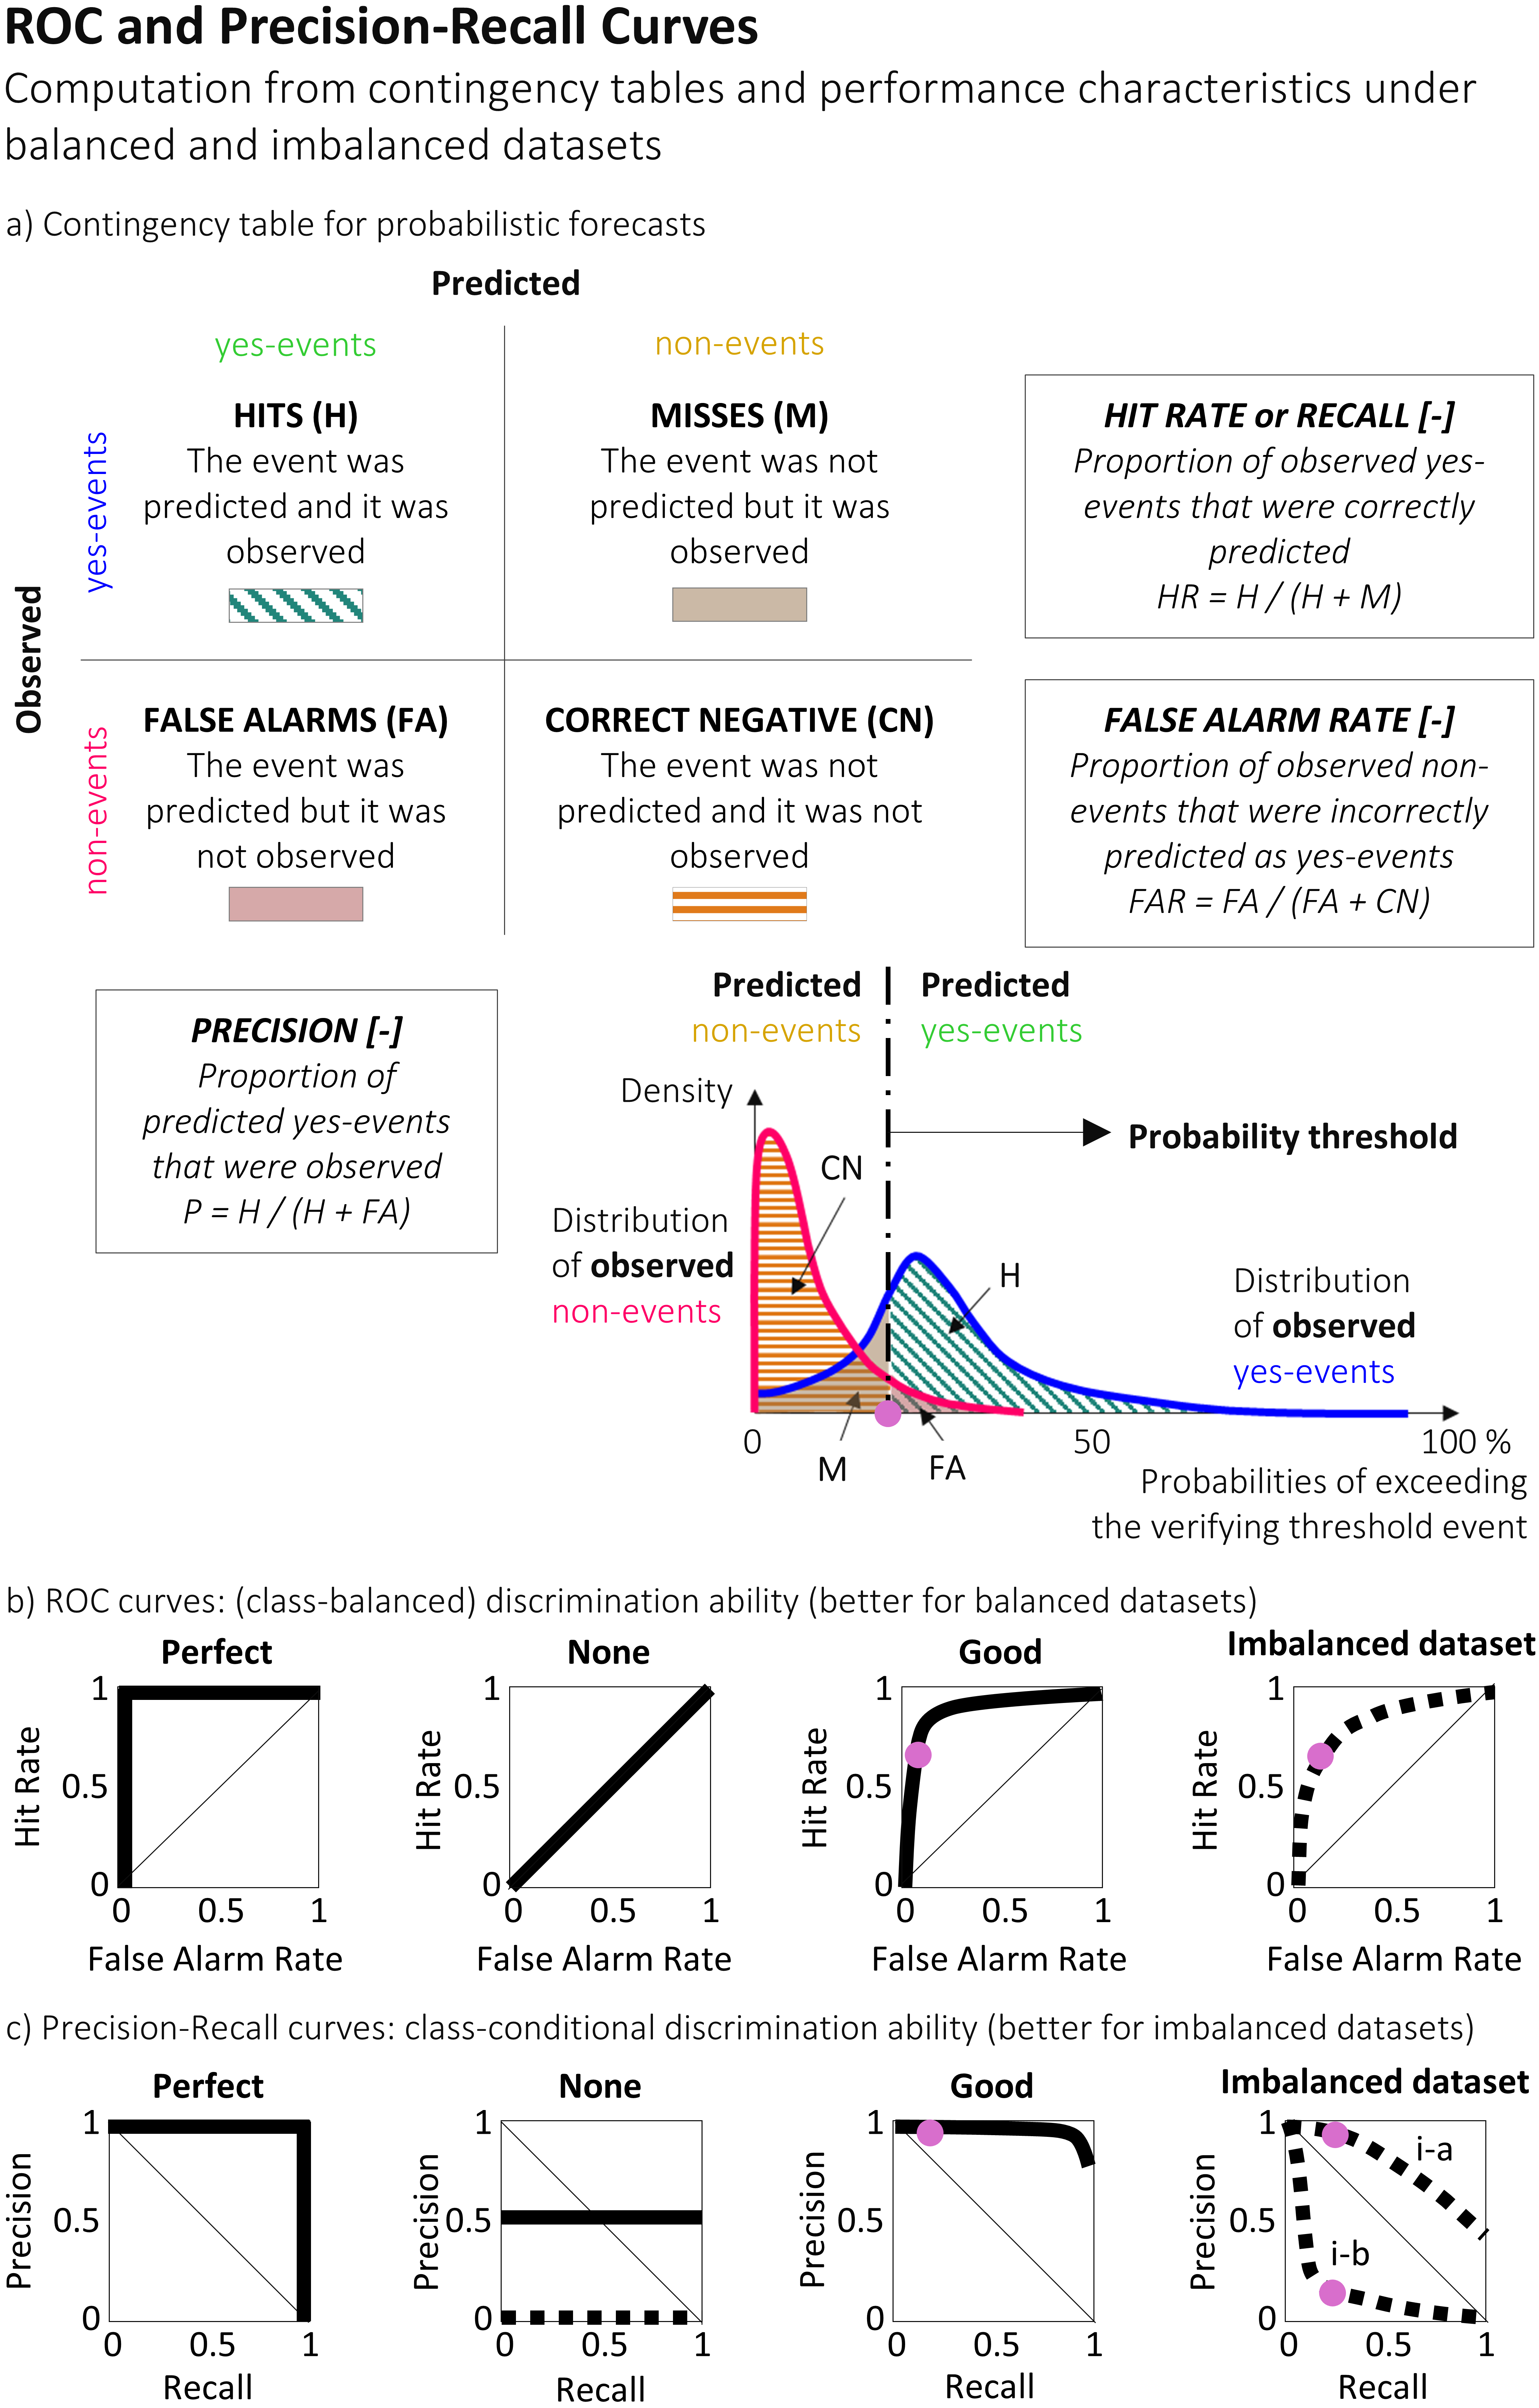
\includegraphics[scale=0.9]{curve_roc_pr_examples.png}
\caption{\textbf{Examples of Receiver Operating Characteristic (ROC) and Precision-Recall curves: computation from contingency tables and performance characteristics under balanced and imbalanced datasets.} Panel (a) defines the four contingency table elements for a binary classification of probabilistic forecasts at a given probability threshold. The probability density plot displays the distribution of observed yes-events (blue) and observed non-events (pink). The vertical dash-dot line passing over a given probability threshold (purple dot) divides the space in predicted yes-events (to the right, in green) and predicted non-events (to the left, in yellow). The overlaps between the two spaces and the density distributions define the elements of the contingency table: H (area covered by dark green sloping lines), FA (area covered by dark pink), M (area covered by dark brown), and CN (area covered by orange horizontal lines). Panel (b) shows how discrimination ability is represented by ROC curves (which assume balance between the binary classes) across different model performances - perfect, none, and good - with the rightmost panel showing discrimination ability for an imbalanced dataset. Panel (c) shows the same as panel (b), but for precision-recall curves (which do not assume class balance between the binary classes).}
\label{fig:curve_roc_pr_examples}
\end{figure}

To \marginpara{Chosen case-studies for subjective verification: flash floods generated by large-scale, widespread rainfall and small-scale, localised rainfall} understand differences in performance and predictability across various flash flood events, it is essential to differentiate between two categories of flash-flood-triggering rainfall: (1) large-scale, widespread rainfall due to persistent moderate-to-extreme stratiform rainfall or short-to-medium duration mesoscale convective systems delivering extreme rainfall, and (2) small-scale, localise rainfall due to short duration convective systems delivering very intense rainfall (see Figure \ref{fig:forecast_evaluatio_strategy}, "Subjective Verification" section). By examining, through well-observed case studies, the forecast performance and predictability of these two categories of flash flood events, it is possible to determine whether deficiencies in predicting areas at risk of flash floods stem from inherent limitations in rainfall forecasting or other factors within the hydrological modelling chain. Hence, each objective verification study in the main analysis chapters (Chapter \ref{flash_flood_focused_verification_rainfall_based_ff} to \ref{data_driven_flash_floods_short_medium_range}) will be complemented with case-study-based subjective verification assessing the performance and predictability of predicting areas at risk of flash floods over large- and small-scale flash-flood-triggering rainfall events.


%%%%%%%%%%%%%%%%%%%%%%%%%%%%%%%%%%%%%%%%%%%%%%%%%%%%%%%%%%%%%%%%%%%%%%%%%%
\section{Data-driven model development strategy 
under imbalanced observational datasets}
\label{integrated_experimental_strategy_model_development_imbalanced_data}

The development of data-driven models that predict areas at risk of flash floods must confront the fundamental challenge of training such models with extremely imbalanced observational datasets. The yes-event class (i.e. when a flash flood event is reported) represents \sim0.2\% of the total number of reports in the database\footnote{For more details on the representation of yes-events in NOAA's Storm Event Database, please refer to Section \ref{datasets_storm_event_database} in Chapter \ref{datasets}}, creating one of the most severe class imbalance problems encountered in environmental prediction, comparable to the detection of lightning \citep{Cavaiola_2024} or landslides \citep{Xu_2022, Agrawal_2017, Zhang_2022, Gupta_2023}. 

\subsection{Requirements to develop robust data-driven models under imbalanced datasets}

At \marginpara{Requirement to develop robust data-driven models under imbalanced datasets n.1: adoption of algorithm-level and ensemble-level approaches for uncertainty quantification in the data-driven predictions} an initial "proof-of-concept" stage, the need for uncertainty quantification to produce robust models should be satisfied by the use of algorithm- and ensemble-level approaches rather than data-level methods. Algorithm-level approaches modify the learning process through techniques such as weighted learning functions, while ensemble-level methods, such as ensemble-based algorithms (e.g., random forest and boosting) or cross-validation, combine multiple classifiers or train many models over different samples of the training dataset to capture the inherent uncertainties in predictions generated with imbalanced observational datasets. In contrast, data-level approaches, also known as sampling methods, include oversampling, undersampling, and synthetic data generation, which modify the training dataset, altering the original ratio between yes- and no-events and, potentially, obscuring the true rarity of flash flood events and compromising uncertainty estimates. By preserving the original ratio in the observational dataset, the developed models provide probability estimates that may reflect actual flash flood occurrence patterns, and prediction uncertainties may remain interpretable for operational decision-making. Whilst more sophisticated sampling methods may prove beneficial in future development stages, this initial proof-of-concept prioritises approaches that maintain data integrity, establishing a baseline against which more complex systems can be benchmarked.

Data-driven \marginpara{Requirement to develop robust data-driven models under imbalanced datasets n.2: select appropriate evaluation metrics to avoid trivial classifiers} models trained on severely imbalanced datasets risk converging to trivial classifiers that can easily achieve accuracy exceeding 99\% by exclusively predicting non-events. Such a system would indeed provide no operational value. Hence, the model development strategy must employ metrics that can extract the most minimal predictive signal (i.e., identify the yes-events) from a sea of noise (i.e., non-events), while maintaining a low count of false alarms.

\subsection{Proposed strategies and implementation}

To \marginpara{Chosen strategy for developing robust data-driven models under imbalanced datasets: ensemble learning algorithms and weighted loss functions} develop robust data-driven models under imbalanced datasets, this thesis employs three distinct approaches. The model development first incorporates multiple ensemble algorithms, including Random Forest, Gradient Boosting variants (XGBoost, LightGBM, CatBoost), and ensemble stacking methods. Each algorithm offers distinct mechanisms for handling imbalanced datasets without requiring data manipulation. Random Forest creates multiple views of the data through bootstrap sampling, potentially improving the representation of positive events in individual trees. Gradient boosting methods sequentially focus on misclassified examples, progressively enhancing detection of difficult-to-predict positive cases. This algorithmic diversity enables a comprehensive assessment of which approaches best capture the subtle signals preceding flash flood events. To train each of these models, this thesis will test two different loss functions: one that weighs all misclassifications equally, effectively obscuring the importance of correctly identifying rare positive events, such as cross-entropy, and one loss function that directly targets imbalanced datasets, such as "weighted cross-entropy". Both sets of forecasts will be evaluated and compared to assess which approach might yield better results. Finally, even though each of the classifiers mentioned above is considered an ensemble technique, the corresponding outputs are created with a deterministic configuration, which says very little about the uncertainty around the predictions and the generalisation performance of the models. Hence, multiple configurations for each classifier (and loss function) will be created by applying the "k-fold cross-validation" approach. Moreover, the consolidated configuration for each classifier will be combined through the "ensemble stacking" technique, a meta-learning technique that optimally blends individual classifier outputs to produce robust final predictions with associated uncertainty estimates.

The \marginpara{Chosen robust evaluation metrics: area under the precision-recall curve (AUPRC) vs. area under the ROC curve (AROC} evaluation framework employs metrics specifically designed for imbalanced classification problems. A commonly used metric consists of the area under the ROC curve (AROC, which balances hit rates and false alarms. As explained in Section \ref{integrated_experimental_strategy_verification_strategy}, AROC is a measure of the prediction's discrimination ability (i.e. the system's ability to distinguish between yes-events and non-events). Since uncalibrated forecasts may yield higher values of AROC by overestimating the probability of flash flood occurrence, choosing this evaluation metric for hyperparameter optimisation or evaluation of forecasts over unseen test data may mean seeking a system that does not miss events, even at the expense of generating more false alarms. Another popular evaluation metric in the domain of data-driven model development is the area under the precision-recall curve. In this case, the focus lies on balancing precision (the fraction of predicted events that materialise) and recall (the fraction of actual events successfully predicted, also known as hit rates). Hence, choosing this evaluation metric may mean seeking a system that provides better-calibrated forecasts to identify yes-events, but by limiting the number of false alarms. The literature remains divided on which of these two popular evaluation metrics is likely to yield the best results \citep{Richardson_2024, Saito_2015}. Hence, this thesis presents results obtained using both evaluation metrics.


%%%%%%%%%%%%%%%%%
\section{Summary}

This chapter has articulated an integrated experimental strategy that systematically addresses the challenge of producing medium-range predictions of areas at risk of flash floods across a continuous global domain. The methodological framework illustrates how seemingly distinct research components converge into a coherent strategy, with each element carefully chosen to support the overarching research questions and objectives in this thesis. The subsequent \textit{Main Analysis} Chapters (\ref{flash_flood_focused_verification_rainfall_based_ff} to \ref{regional_to_global_training}) will implement this integrated experimental strategy, progressively building from fundamental verification principles through regional model development of short- and medium-range forecasts, to the extension of predictions over a continuous global domain.